%%%%%%%% ICML 2021 EXAMPLE LATEX SUBMISSION FILE %%%%%%%%%%%%%%%%%

\documentclass{article}

% Recommended, but optional, packages for figures and better typesetting:
\usepackage{microtype}
\usepackage{graphicx}
\usepackage{amssymb,amsmath}
\usepackage{subfigure}
\usepackage{booktabs} % for professional tables

\newtheorem{definition}{Definition}
\DeclareMathOperator*{\argmin}{arg\, min} 
% hyperref makes hyperlinks in the resulting PDF.
% If your build breaks (sometimes temporarily if a hyperlink spans a page)
% please comment out the following usepackage line and replace
% \usepackage{icml2021} with \usepackage[nohyperref]{icml2021} above.
\usepackage{hyperref}

% Attempt to make hyperref and algorithmic work together better:
\newcommand{\theHalgorithm}{\arabic{algorithm}}

% Use the following line for the initial blind version submitted for review:
\usepackage{icml2021}

% If accepted, instead use the following line for the camera-ready submission:
%\usepackage[accepted]{icml2021}

% The \icmltitle you define below is probably too long as a header.
% Therefore, a short form for the running title is supplied here:
\icmltitlerunning{Submission and Formatting Instructions for ICML 2021}

\begin{document}

\twocolumn[
\icmltitle{Gradient-based Optimization of the Area Under the Minimum of False Positive and False Negative Functions}

% It is OKAY to include author information, even for blind
% submissions: the style file will automatically remove it for you
% unless you've provided the [accepted] option to the icml2021
% package.

% List of affiliations: The first argument should be a (short)
% identifier you will use later to specify author affiliations
% Academic affiliations should list Department, University, City, Region, Country
% Industry affiliations should list Company, City, Region, Country

% You can specify symbols, otherwise they are numbered in order.
% Ideally, you should not use this facility. Affiliations will be numbered
% in order of appearance and this is the preferred way.
\icmlsetsymbol{equal}{*}

\begin{icmlauthorlist}
\icmlauthor{Aeiau Zzzz}{equal,to}
\icmlauthor{Bauiu C.~Yyyy}{equal,to,goo}
\icmlauthor{Cieua Vvvvv}{goo}
\icmlauthor{Iaesut Saoeu}{ed}
\icmlauthor{Fiuea Rrrr}{to}
\icmlauthor{Tateu H.~Yasehe}{ed,to,goo}
\icmlauthor{Aaoeu Iasoh}{goo}
\icmlauthor{Buiui Eueu}{ed}
\icmlauthor{Aeuia Zzzz}{ed}
\icmlauthor{Bieea C.~Yyyy}{to,goo}
\icmlauthor{Teoau Xxxx}{ed}
\icmlauthor{Eee Pppp}{ed}
\end{icmlauthorlist}

\icmlaffiliation{to}{Department of Computation, University of Torontoland, Torontoland, Canada}
\icmlaffiliation{goo}{Googol ShallowMind, New London, Michigan, USA}
\icmlaffiliation{ed}{School of Computation, University of Edenborrow, Edenborrow, United Kingdom}

\icmlcorrespondingauthor{Cieua Vvvvv}{c.vvvvv@googol.com}
\icmlcorrespondingauthor{Eee Pppp}{ep@eden.co.uk}

% You may provide any keywords that you
% find helpful for describing your paper; these are used to populate
% the "keywords" metadata in the PDF but will not be shown in the document
\icmlkeywords{Machine Learning, ICML}

\vskip 0.3in

]

% this must go after the closing bracket ] following \twocolumn[ ...

% This command actually creates the footnote in the first column
% listing the affiliations and the copyright notice.
% The command takes one argument, which is text to display at the start of the footnote.
% The \icmlEqualContribution command is standard text for equal contribution.
% Remove it (just {}) if you do not need this facility.

%\printAffiliationsAndNotice{}  % leave blank if no need to mention equal contribution
%\printAffiliationsAndNotice{\icmlEqualContribution} % otherwise use the standard text.

\begin{abstract}
Receiver Operating Characteristic (ROC) curves are plots of true positive rate versus false positive rate which are useful for evaluating binary classification models.
ROC curves can also be used in other problems that have false positive and true positive rates such as changepoint detection.
We show that in this more general context, the ROC curve is not always monotonic, and so if loops are present the Area Under the Curve (AUC) can be greater than one.
Instead of maximizing the AUC for these problems, we propose to minimize a new loss function called the AUM, short for Area Under Min(FP, FN).
We show that the AUM gradient can be efficiently computed and used in a new gradient descent learning algorithm.
In our empirical study of supervised changepoint detection problems, we show that AUM minimization results in improved AUC relative to previous baselines.
\end{abstract}

\section{Introduction}
\label{sec:introduction}
In machine learning problems such as supervised binary classification and changepoint detection, the goal is to learn a function for accurately predicting presence or absence of a class label.
In binary classification there is a prediction for each example; in changepoint detection there is a prediction (change or not) in between each data point in a sequence.
%Our main goal in this research project is to generate a linear model that yields a higher model performance than previously baseline linear models. 
There are numerous ways to analyze a model's performance, but the simplest way is to calculate its accuracy, which is the number or proportion of correctly classified labels.
However using accuracy as the evaluation metric can be problematic for data sets with imbalanced labels or for which the desired weighting of the labels is unknown.
% For example, consider a data set with a high number of positive labels.
% One could generate a model with a high accuracy simply by predicted every label to be positive, without any consideration of the features of the instance.
% This model is essentially useless, as it would never be capable of predicting when an example may have a negative label. 

A popular approach for comparing models in this context is by analyzing Receiver Operating Characteristic (ROC) curves, which are plots of True Positive Rate (TPR) versus False Positive Rate (FPR).
A single prediction vector for model can be visualized as a single point in ROC space; the ROC curve is traced by adding a constant real-valued threshold to each prediction in that vector.
Large thresholds result in FPR=TPR=1 and small thresholds result in FPR=TPR=0.
Therefore the Area Under the Curve (AUC) is an evaluation metric which accounts for all possible thresholds or weights for the class labels.
In typical binary classification problems, a perfect model has an AUC of 1, a random/baseline model has an AUC of 0.5, and the minimum AUC is 0.

When AUC is used as the evaluation metric in machine learning, the best algorithm is defined as the one that maximizes test AUC (in cross-validation on a specific data set).
In such experiments we would also like to use the AUC as the objective function for training the model (under the assumption that if the train and test sets are similar, maximizing train AUC should result in maximizing test AUC). 
However, since the AUC is a piecewise constant function of the predicted values, its gradient is zero almost everywhere, and it is therefore impossible to directly optimize using gradient descent algorithms.

In this paper we study supervised changepoint detection, in which we can compute FPR and TPR as in binary classification.
For binary classification we can compute a prediction vector which maximizes AUC in the same way as maximizing accuracy --- predict a positive value for each positive label, and a negative value for each negative label.
For changepoint detection it is also trivial to compute a prediction vector that maximizes accuracy, but it can be non-trivial to compute a prediction vector that maximizes AUC (even for an unconstrained model on the train set).
This is because in changepoint detection the FPR and TPR may be non-monotonic functions of the predicted values, which means that the ROC curve may have loops.

\subsection{Contributions}

The previous observations motivate our current paper, which explores a new loss function and corresponding optimization algorithm for problems like binary classification and changepoint detection.
In particular, we study the minimum of false positive and false negative counts as a function of the prediction threshold.
We propose the Area Under the Minimum (AUM) as a new loss function for use in supervised learning algorithms.
We give an efficient algorithm for computing directional derivatives of the AUM with respect to predicted values, which we propose using in gradient descent learning algorithms.
Our empirical study of supervised changepoint detection problems shows that minimizing the AUM corresponds to maximizing the AUC (with respect to train and test sets).

\begin{figure*}[ht]
\vskip 0.2in
\begin{center}
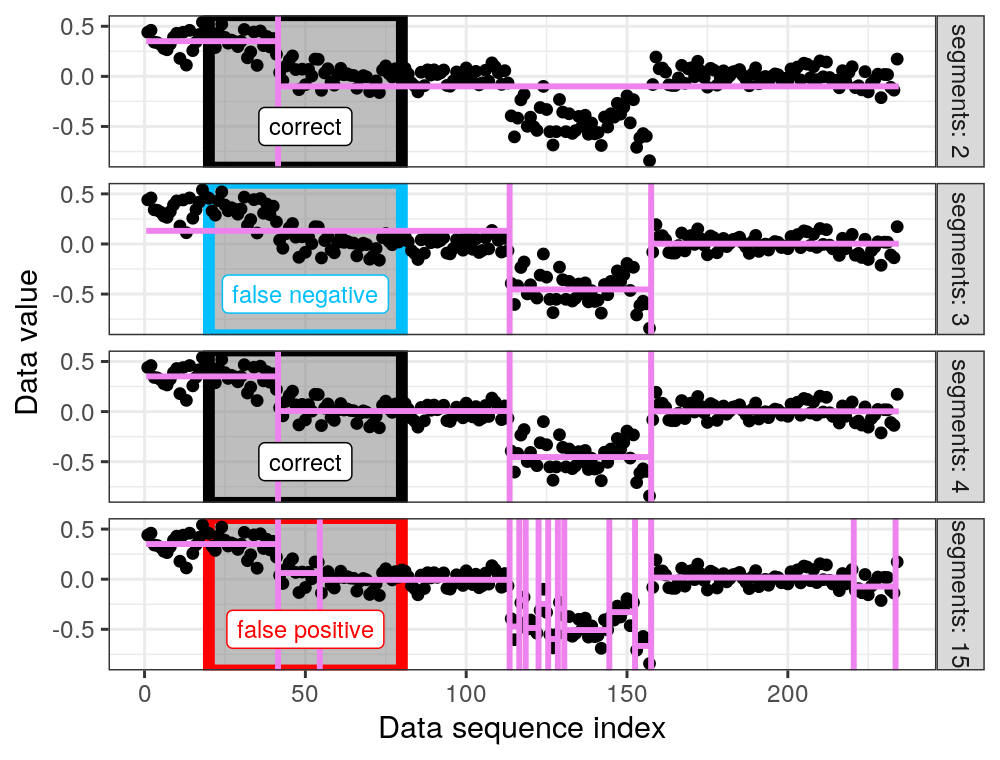
\includegraphics[width=0.59\textwidth]{figure-fn-not-monotonic.png}
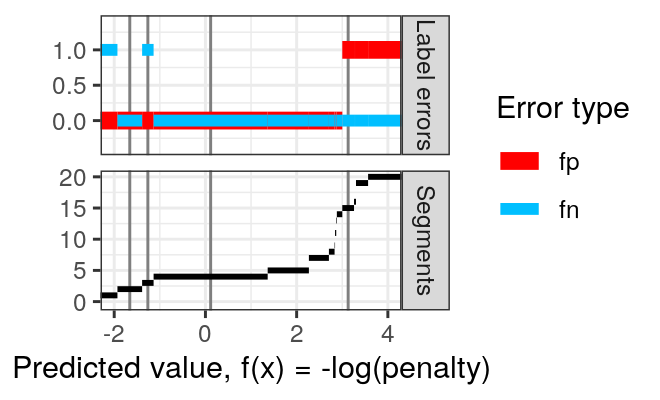
\includegraphics[width=0.4\textwidth]{figure-fn-not-monotonic-error.png}
\vskip -0.5cm
\caption{Example data for which the ROC curve is non-monotonic. 
\textbf{Left:} a data sequence (black dots) with one label (grey rectangle) in which there should be exactly one predicted changepoint (false negative for no changes when segments=3, false positive for two changes when segments=15).  
\textbf{Right:} selected number of segments (bottom) and number of label errors (top) as a function of predicted values $f(x)$, with vertical grey lines indicating the models shown on the left. Note how the fn function is not monotonic.c
}
\label{fig:fn-not-monotonic}
\end{center}
\vskip -0.2in
\end{figure*}


\subsection{Related work}
\label{sec:related-work}

TODO Jon citations

Related work on AUC optimization falls into two categories: gradient
learning algorithms based on re-weighting or approximation, and
discrete learning algorithms such as decision trees.
\citet{ferri2002learning} proposed expressions for the expected value
and the variance of the AUC for a fixed error rate, in the context of
a decision tree learning algorithm called AUCsplit.
\citet{yan2003optimizing} proposed a global approximation of AUC which was then used in several other algorithms.
For example, \citet{castro2008optimization} used that approxmation to propose the AUCtron algorithm which learns a linear model.
Other algorithms have been proposed to obtain approximations of the global AUC value \citep{yan2003optimizing, rakotomamonjy2004optimizing, herschtal2004optimising, herschtal2006area}.
\citet{Han2010} proposed an active learning algorithm for computing a linear model that maximizes the AUC.

\section{Models and Definitions}
\label{sec:model}
We begin by reviewing supervised binary classification and changepoint detection, then give definitions for AUC and the new AUM loss function.
\subsection{Review of supervised binary classification}

In supervised binary classification we are given a set of $n$ labeled training examples, $\{(\mathbf x_i, y_i)\}_{i=1}^n$ where $\mathbf x_i\in\mathbb R^p$ is an input feature vector for one observation and $y_i\in\{-1,1\}$ is a binary output/label.
The goal of binary classification is to learn a function $f:\mathbb R^p\rightarrow \mathbb R$ which outputs a real-valued prediction with the same sign as the corresponding label.
Learning algorithms such as logistic regression and support vector machines involve minimizing a convex loss function $\ell:\mathbb R\times \{-1,1\}$, summed over all training examples:
\begin{equation}
\label{eq:loss-sum-over-examples}
    \mathcal L(f) =  \sum_{i=1}^n \ell[ f(\mathbf x_i), y_i].
\end{equation}
After a function $f$ has been learned using the training data, it can be evaluated by computing non-convex evaluation metrics such as the zero-one loss or the AUC with respect to a held-out test set.

\subsection{Review of supervised changepoint detection}

In supervised changepoint detection \citep{Hocking2013icml}, we have  $n$ labeled training examples. 
Each labeled training example $i\in\{1,\dots,n\}$ has a corresponding data sequence vector $\mathbf z_i$ and label set $L_i$.
For example in Figure~\ref{fig:fn-not-monotonic} we show a data sequence $\mathbf z_i$ with a label set $L_i$ that contains one positive label (grey region in which there should be exactly one predicted changepoint).
Dynamic programming algorithms can be used on the data sequence $\mathbf z_i$ to compute a path of optimal changepoint models $\mathbf {\hat m}^k_i$ for different model sizes $k\in\{1,2,\dots\}$  \citep{Maidstone2016}.
For example in Figure~\ref{fig:fn-not-monotonic} (left) we show four models in the path (with 2,3,4,15 segments).
The label set $L_i$ can be used to compute the number of false positive and false negative labels with respect to any predicted set of changepoints (false positives for too many changepoints, false negatives for not enough changepoints).
Each example $i$ also has a model selection function $k^*_i:\mathbb R^+_0 \rightarrow \{1,2,\dots\}$ which map a non-negative penalty value $\hat \lambda_i$ to a selected model size $k^*_i(\hat \lambda_i)$ (Figure~\ref{fig:fn-not-monotonic}, right bottom).
We assume there is a fixed feature map $\phi$ which can be used to compute a feature vector $\mathbf x_i = \phi(\mathbf z_i)\in\mathbb R^p$ for each labeled example.

We want to learn a function $f:\mathbb R^p\rightarrow \mathbb R$ which inputs a feature vector and outputs a real-valued prediction that is used as a negative log penalty value, $f(\mathbf x_i) = -\log \hat \lambda_i$.
The goal is to predict model sizes $k^*_i(\hat \lambda_i)$ that result in minimal label errors. 
Since the label error function is non-convex like the zero-one loss in binary classification (Figure~\ref{fig:fn-not-monotonic}, right top), the learning algorithm instead uses gradient descent on a convex squared hinge loss \citep{Hocking2013icml}, as in (\ref{eq:loss-sum-over-examples}).

\begin{figure*}[ht]
\vskip 0.2in
\begin{center}
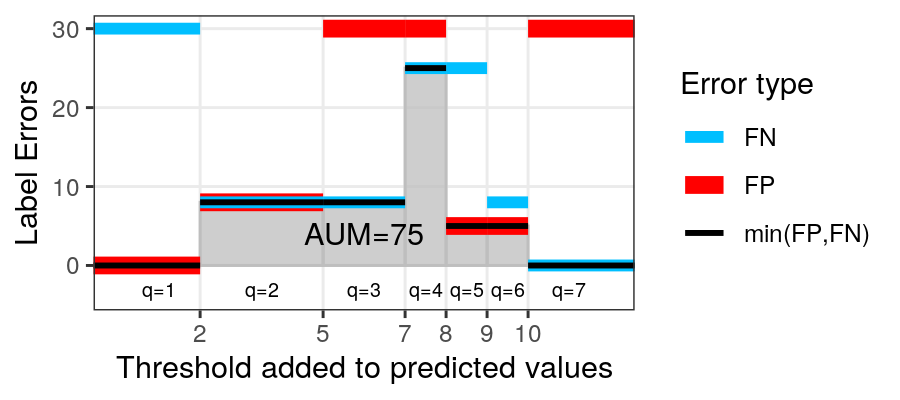
\includegraphics[width=0.55\textwidth]{figure-more-than-one-more-aum.png}
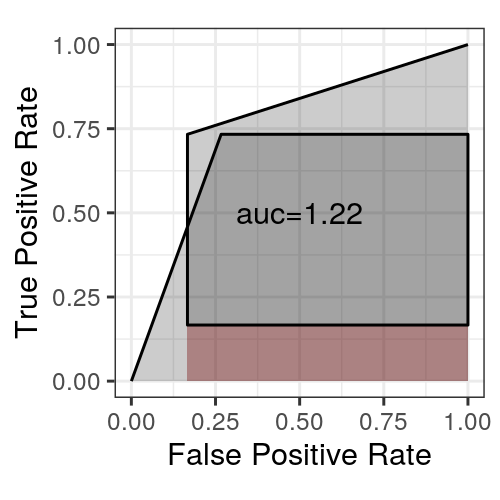
\includegraphics[width=0.25\textwidth]{figure-more-than-one-more-auc.png}
\vskip -0.5cm
\caption{Synthetic example showing how non-monotonic fp/fn functions (left) result in looping ROC curves (right). 
\textbf{Left:} the aum (grey area) is defined as the area under the minimum of fp and fn functions.
\textbf{Right:} the auc is more than 1 due to the loop which results in double counting the dark grey area (but single counting the red area which is positive counted twice and negative counted once).
}
\label{fig:more}
\end{center}
\vskip -0.2in
\end{figure*}

\subsection{Definition of false positive and negative functions}

%Now we assume that $n$ is the number of related problems for which we want to make a real-valued prediction (same as the number of labeled training examples in binary classification).
%For each problem $i \in \{1, 2, \dots n\}$, we make a real-valued prediction $f(\mathbf x_i) = \hat y_i\in\mathbb R$, and let $\mathbf{ \hat y}$ be the $n$-dimensional vector with $\hat y_i$ in each coordinate $i\in\{1,\dots,n\}$.

In this paper we assume the following general learning context in which supervised binary classification and changepoint detection are specific examples. 
For each labeled training example $i$, we have one or more labels such that there are at most $\text{FNP}_i\in\mathbb Z_+=\{0, 1, \dots\}$  false negatives possible and $\text{FPP}_i\in\mathbb Z_+$ false positives possible.
Given a real-valued prediction $\hat y_i=f(\mathbf x_i)\in\mathbb R$, we can use the labels to compute the number of predicted false positives $\text{FP}_i(\hat y_i)\in \{0, \dots, \text{FPP}_i\}$ and false negatives $\text{FN}_i(\hat y_i)\in\{0, \dots, \text{FNP}_i\}$.
The $\text{FP}_i,\text{FN}_i$ functions return the number of false positive and false negative labels for a given predicted value $\hat y_i$. 
By convention we assume the $\text{FP}_i,\text{FN}_i$ functions are right continuous.
We furthermore assume that $\text{FP}_i(-\infty)=0$ and $\text{FN}_i(\infty)=0$ (so that our proposed AUM loss function is always finite).

In the case of binary classification, for all positive examples $i:y_i=1$ we have 
\begin{eqnarray}
  \text{FPP}_i&=&0,\\
  \text{FNP}_i&=&1, \\
  \text{FP}_i(\hat y) &=& 0, \\
  \text{FN}_i(\hat y) &=& I(\hat y < 0),
\end{eqnarray}
where $I$ is the indicator function (outputs 1 if argument is true, 0 otherwise).
For all negative examples $i:y_i=-1$,
\begin{eqnarray}
  \text{FPP}_i&=&1,\\
  \text{FNP}_i&=&0, \\
  \text{FP}_i(\hat y) &=& I(\hat y \geq 0), \\
  \text{FN}_i(\hat y) &=& 0.
\end{eqnarray}
Note that $\text{FP}_i$ is either constant/zero (for positive examples) or non-decreasing (for negative examples), and $\text{FN}_i$ is either constant/zero (for negative examples) or non-increasing (for positive examples).

In changepoint detection we have more general $\text{FP}_i$ and $\text{FN}_i$ functions that can be non-monotonic.
For example in Figure~\ref{fig:fn-not-monotonic} we show a data sequence with one positive label (in which there should be exactly one predicted changepoint).
Predicting no changepoint in this label results in a false negative, and predicting two changepoint in this label results in a false positive. 
Therefore, we have $\text{FPP}_i=\text{FNP}_i=1$ for this particular example $i$;
% > err.list$model.errors[, .(min.log.lambda, max.log.lambda, segments, fp, fn)]
%     min.log.lambda max.log.lambda segments fp fn
%  1:           -Inf      -3.566634       20  1  0
%  2:      -3.566634      -3.301154       19  1  0
%  3:      -3.301154      -3.258186       16  1  0
%  4:      -3.258186      -3.000918       15  1  0
%  5:      -3.000918      -2.881569       14  0  0
%  6:      -2.881569      -2.868007       13  0  0
%  7:      -2.868007      -2.842141       11  0  0
%  8:      -2.842141      -2.831636        9  0  0
%  9:      -2.831636      -2.707501        8  0  0
% 10:      -2.707501      -2.268619        7  0  0
% 11:      -2.268619      -1.365036        5  0  0
% 12:      -1.365036       1.136433        4  0  0
% 13:       1.136433       1.388073        3  0  1
% 14:       1.388073       1.929300        2  0  0
% 15:       1.929300            Inf        1  0  1
the false positive function is non-decreasing, $\text{FP}_i(\hat y_i) \approx I(\hat y_i \geq 3)$, and the false negative function is not monotonic, $\text{FN}_i(\hat y_i) \approx I[\hat y_i \in (\infty, -1.9)\cup [-1.4, -1.1)]$.
When the false negative function is non-monotonic, the true positive rate is also non-monotonic (the ROC curve can move down as well as up).

\subsection{Definition of ROC curve and AUC}

In this section we show how the previously defined functions can be used to define the ROC curve and the AUC.

%Let $f : \mathbb R^p \rightarrow \mathbb R$ be the function we want to learn, which maps feature vectors to real-valued predictions, e.g. $\hat y_i = f(X_i)$ for all $i \in \{1, \dots, n\}$. $t \in \mathbb{R}$ is a threshold value that is added onto each of the predictions before a final label is produced.

% The total number of label errors is a function which can be summed over observations, 
% \begin{equation}
%     E(\hat y_1, \dots, \hat y_n) = 
%     \sum_{i=1}^n \text{FP}_i(\hat y_i) + \text{FN}_i(\hat y_i).
% \end{equation}


\begin{figure*}[ht]
\vskip 0.2in
\begin{center}
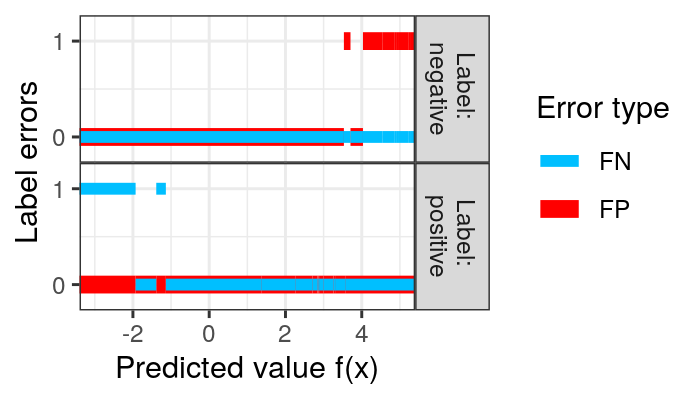
\includegraphics[height=4cm]{figure-aum-convexity-profiles.png}
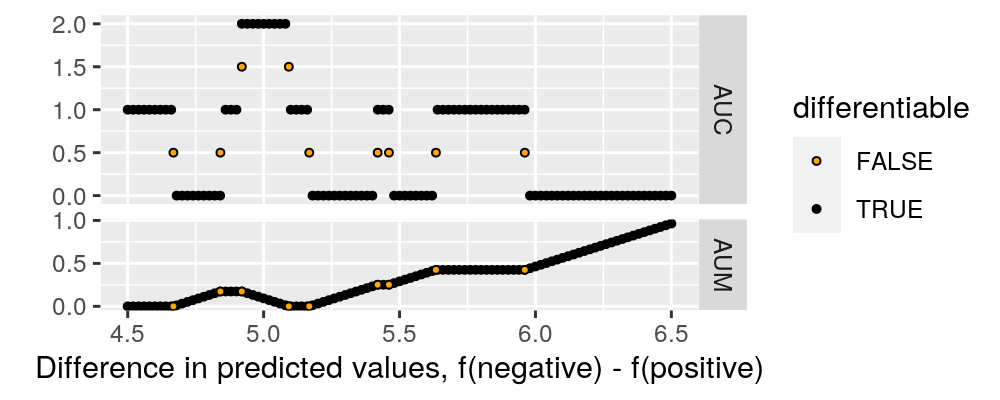
\includegraphics[height=4cm]{figure-aum-convexity.png}
\vskip -0.5cm
\caption{Real data example showing that it is possible to have AUC greater than one.
\textbf{Left:} error functions for two labeled examples in a real changepoint detection data set.
\textbf{Right:} AUM and AUC values as a function of the difference in predicted values between the two labeled examples.
When the difference is around 5, we have AUC=2.
We can see that the AUC is a piecewise constant function of the predicted values, whereas the AUM is a continuous piecewise linear function.
It can be seen in this example that at differentiable points, AUM=0 implies AUC=1 (but the converse is false).
}
\label{fig:aum-convexity}
\end{center}
\vskip -0.2in
\end{figure*}

Given a vector of predictions $\mathbf{\hat y}$, we define the False Positive Total (FPT) and False Negative Total (FNT) over all labeled examples $i$ as
\begin{eqnarray}
 \text{FPT}(\mathbf {\hat y}) &=&
 \sum_{i} \text{FP}_i(\hat y_i) \\
 \text{FNT}(\mathbf {\hat y}) &=&
 \sum_{i} \text{FN}_i(\hat y_i) 
\end{eqnarray}
For a prediction threshold $t\in\mathbb R$ we define the False Positive Rate (FPR), False Negative Rate (FNR), and True Positive Rate (TPR) functions as
\begin{eqnarray}
 \text{FPR}_{\mathbf {\hat y}}(t) &=&
 \frac{1}{\sum_i \text{FPP}_i } 
 \text{FPT}(\mathbf {\hat y}+t), \\
 \text{FNR}_{\mathbf {\hat y}}(t) &=&
 \frac{1}{\sum_i \text{FNP}_i } 
 \text{FNT}(\mathbf {\hat y}+t),\\
 \text{TPR}_{\mathbf {\hat y}}(t) &=&
 1 - \text{FNR}_{\mathbf {\hat y}}(t)
\end{eqnarray}
The ROC curve for a given prediction vector $\mathbf {\hat y}$ is the plot of $\text{TPR}_{\mathbf {\hat y}}(t) $ versus $\text{FPR}_{\mathbf {\hat y}}(t) $ as the prediction threshold $t$ is varied from $-\infty$ to $\infty$.
The AUC can be written as an integral,
\begin{equation}
    \text{AUC}(\mathbf{\hat y}) = 
    \int \text{TPR}_{\mathbf {\hat y}}(t) 
    d\, \text{FPR}_{\mathbf{\hat y}}(t).
\end{equation}
Assuming the $\text{FPT}$ and $\text{FNT}$ functions are piecewise constant (as in binary classification and changepoint detection) then the ROC curve can be described as a sequence of $Q$ points 
$\{(\text{fpr}
(\mathbf {\hat y})
_q, \text{tpr}
(\mathbf {\hat y})
_q)\}_{q=1}^Q$ in ROC space (note that this sequence of points depends on the predicted values $\mathbf {\hat y}$).
The first point $q=1$ corresponds to prediction threshold $t=-\infty$ which results in TPR=0 and FPR=0; the last point $q=Q$ is for $t=\infty$ which results in TPR=1 and FPR=1.
The AUC can be computed using this sequence,
\begin{eqnarray}
\label{eq:auc-seq}
&&\text{AUC}(\mathbf {\hat y}) = \\
  &&  \sum_{q=1}^{Q-1} 
    (\text{fpr}
    (\mathbf {\hat y})
    _{q+1} - \text{fpr}
    (\mathbf {\hat y})
    _q)
    (\text{tpr}
    (\mathbf {\hat y})
    _{q} + \text{tpr}
    (\mathbf {\hat y})
    _{q+1})/2.\nonumber
\end{eqnarray}
In binary classification we have $\text{fpr}(\mathbf {\hat y})_{q} \leq \text{fpr}(\mathbf {\hat y})_{q+1}$ which means while tracing the ROC curve there are no moves to the left, and all the terms in the sum above are positive.
In fact this is also true of changepoint detection problems for which all the $\text{FP}_i$ functions are non-decreasing. 
In these cases the ROC curve is monotonic, with $\text{AUC}(\mathbf {\hat y})\in[0,1]$ for any predicted values $\mathbf {\hat y}$.

\subsection{Existence of non-monotonic ROC curves}

However if some of the $\text{FP}_i$ functions are not monotonic, then it is possible to have $\text{fpr}(\mathbf {\hat y})_{q} > \text{fpr}(\mathbf {\hat y})_{q+1}$ which results in negative terms in the AUC equation~(\ref{eq:auc-seq}). 
Furthermore if some of the $\text{FN}_i$ functions are not monotonic, then the ROC curve can contain loops which double count some area in ROC space.
For a simple synthetic example, consider the FP/FN functions and corresponding ROC curves in Figure~\ref{fig:more}.
In this example, the ROC curve contains one loop which results in double counting a large portion of ROC space, which results in an AUC value greater than one.


But does this happen in real data? Yes, in real changepoint detection problems such as Figure~\ref{fig:fn-not-monotonic} it is clearly possible to have error functions which are non-monotonic.
Furthermore, in Figure~\ref{fig:aum-convexity} we show error curves for two labeled examples from another real changepoint detection data set.
One example has a positive label that results in a non-monotonic false negative function, and the other example has a negative label that results in a non-monotonic false positive function.
In general with non-monotonic false positive and false negative functions, it is not clear how to compute predictions which result in max AUC.
However since there are only two labeled examples in this case, we can do grid search over the difference in predicted values.
When the predicted value for the negative example is about 5 greater than the predicted value for the positive example, we observe AUC=2.

This begs the question, is it desirable to maximize the AUC? If so then how can it be maximized efficiently? If not then should we optimize some other criterion?
In typical binary classification problems it is desirable to maximize the AUC because of the ROC curve is monotonic, which means that each point on the curve is an optimal tradeoff between true positive and false positive rates (for a given threshold or weighting of positive versus negative examples).
However in this more general context it is no longer true that each point on the ROC curve results in an optimal tradeoff --- when there are loops there are thresholds which are clearly sub-optimal in terms of TPR and/or FPR.

\subsection{Proposed loss function: AUM}

In this section we propose the AUM loss function, which is short for Area Under Min(FP,FN).
First we must define the minimum of total false positives and false negatives, 
\begin{equation}
    M(\mathbf {\hat y}) = 
    \min\{
    \text{FPT}(\mathbf{\hat y}),
    \text{FNT}(\mathbf{\hat y})
    \}.
\end{equation}
Then we define the AUM as 
\begin{equation}
\label{eq:AUM}
    \text{AUM}(\mathbf {\hat y}) =
    \int_{-\infty}^{\infty}
    M(\mathbf {\hat y} + t)\, dt.
\end{equation}
In summary, we compute AUM by integrating the $M$ function over all possible prediction thresholds $t$.
Geometrically, this corresponds to the area under the minimum of total false positive and false negative functions (Figure~\ref{fig:more}, left).
Since $M$ is the minimum of the total false positives and false negatives over all examples, a few interesting properties should be immediately apparent.
\begin{description}
    \item[Finite.] 
First, since $\text{FP}_i(-\infty)=0$ and $\text{FN}_i(\infty)=0$ (by assumption), we have $M(\mathbf{\hat y}\pm\infty)=0$, which means the minimum is zero at both extreme prediction thresholds. 
Therefore the AUM integral~(\ref{eq:AUM}) is finite, $\text{AUM}(\mathbf{\hat y})<\infty$.
\item[Non-negative.] Second, because the label error functions are never negative, the AUM integral is never negative, $\text{AUM}(\mathbf{\hat y})\geq 0$.
\item[Zero condition.] Third, we have $\text{AUM}(\mathbf{\hat y})=0$ if and only if $M(\mathbf{\hat y}+t)=0$ for all thresholds $t$.
\item[Other properties.] The AUM is a continuous, piecewise linear, non-convex function which is differentiable almost everywhere. 
\end{description}
Exploring the precise relationship between AUM and AUC is an interesting direction for future theoretical work.
In particular we have observed empirically that the  non-differentiable points in the AUM coincide with discontinuities in AUC (Figure~\ref{fig:aum-convexity}, right).
Furthermore we observed that at differentiable points, 
if $\text{AUM}(\mathbf{\hat y})=0$ then
$\text{AUC}(\mathbf{\hat y})=1$; 
the converse is clearly false, however (Figure~\ref{fig:aum-convexity}, right).
This observation suggests that minimizing the AUM would result in a model with AUC=1, so we propose an AUM gradient descent algorithm in the next section.

\section{Algorithms}
\label{sec:algorithms}

In this previous section we have defined the AUM, which we propose to use as a new loss function in supervised learning.
In this section, we propose algorithms for efficiently computing the AUM gradient and for learning a linear model.

\subsection{Exact AUM computation}

%   aum <- fp.fn.totals[, sum(ifelse(
%     min.fp.fn==0, 0, min.fp.fn*(max.thresh-min.thresh)))]
Computing the AUM is similar to the AUC. 
If the $\text{FP}_i,\text{FN}_i$ have an exact representation (in terms of breakpoints in the piecewise constant functions), then we can compute an exact AUM value as follows.
First let $\{(
\text{fpt}
(\mathbf {\hat y})
_q, \text{fnt}
(\mathbf {\hat y})
_q,
 \tau
(\mathbf {\hat y})
_q
)\}_{q=1}^Q$ 
be a sequence of $Q$ tuples, each of which corresponds to a point on the ROC curve.
The fpt/fnt are false positive/negative totals whereas $\tau$ are prediction threshold values 
% which we assume are increasing, $\tau
% (\mathbf {\hat y})
% _q < \tau
% (\mathbf {\hat y})
% _{q+1}$.
which we assume are increasing, $ -\infty = \tau
(\mathbf {\hat y})
_0 < \cdots <  \tau
(\mathbf {\hat y})
_Q = \infty$.
For each $q\in\{1,\dots,Q\}$ we have 
$\text{FPT}(\mathbf{\hat y}+t)=\text{fpt}(\mathbf {\hat y})_q$
and
$\text{FNT}(\mathbf{\hat y}+t)=\text{fnt}(\mathbf {\hat y})_q$
for all $t\in(\tau(\mathbf {\hat y})_{q-1}, \tau(\mathbf {\hat y})_q)$.
Then we define $m(\mathbf {\hat y})_q = \min\{
    \text{fpt}(\mathbf {\hat y})_q , \, 
    \text{fnt}(\mathbf {\hat y})_q
\}$ and so since 
$m(\mathbf {\hat y})_1=m(\mathbf {\hat y})_Q=0$ the AUM can be computed via
\begin{equation}
\label{eq:AUM-computation}
    \text{AUM}(\mathbf {\hat y}) =
    \sum_{q=2}^{Q-1}
    [ \tau(\mathbf {\hat y})_{q} - \tau(\mathbf {\hat y})_{q-1} ]
    m(\mathbf {\hat y})_q.
\end{equation}
For example, in Figure~\ref{fig:more} there are $Q=7$ tuples (points on the ROC curve), five of which result in a non-negative AUM; total AUM is 75.

\subsection{Gradient computation}
\label{sec:gradient-computation}

First we note that the AUM function is not differentiable everywhere, so the gradient is not defined everywhere.
Second we note that the AUM function is non-convex, which means that the sub-differential from convex analysis is not defined \citep{rockafellar-1970a}.
Instead, we propose an algorithm for computing the AUM directional derivatives, which are defined everywhere. 
We recall the general definition of a directional derivative.

\begin{definition}
Given vectors $\mathbf x,\mathbf v\in\mathbb R^n$ and a function $f:\mathbb R^n\rightarrow \mathbb R$, the directional derivative of $f$ at $\mathbf x$ in the direction of $\mathbf v$ is the function $\nabla_{\mathbf v} f: \mathbb R^n \rightarrow \mathbb R$ given by
\begin{equation}
\label{eq:directional-derivative}
    \nabla_{\mathbf v} f(\mathbf x) = 
    \lim_{h\rightarrow 0}
    \frac{f(\mathbf x + h\mathbf v) - 
    f(\mathbf x)}{h}.
\end{equation}
\end{definition}
We would like to compute $\nabla_{\mathbf v}\text{AUM}(\mathbf{\hat y})$, for a set of directions $\mathbf v$.
We are interested in computing the directional derivative along a single dimension $i\in\{1,\dots,n\}$, in either the positive or negative direction, which correspond to using direction vectors $\mathbf v$ with 1 or $-1$ at the $i$-th position, and zeros at each other position, 
\begin{eqnarray}
\mathbf v(1, i) &=& \left[\begin{array}{ccccc}
0 & \cdots & 1 & \cdots & 0
\end{array}\right]^\intercal,
\\
\mathbf v(-1, i) &=& \left[\begin{array}{ccccc}
0 & \cdots & -1 & \cdots & 0
\end{array}\right]^\intercal.
\end{eqnarray}
The intuition of these direction vectors is that each will give us the rate of change of AUM, if a single prediction $i$ is either increased or decreased.
We propose an algorithm for efficiently computing the following $n\times 2$ matrix of directional derivatives,
\begin{equation}
\mathbf D_f(\mathbf x) = 
    \left[\begin{array}{ccc}
\nabla_{\mathbf v(-1,1)} f(\mathbf x) &
\cdots &
\nabla_{\mathbf v(-1,n)} f(\mathbf x) \\
\nabla_{\mathbf v(1,1)} f(\mathbf x) &
\cdots &
\nabla_{\mathbf v(1,n)} f(\mathbf x) 
    \end{array}\right]^\intercal.
\end{equation}
We will compute $\mathbf D_\text{AUM}(\mathbf {\hat y})$, which is the matrix of directional derivatives for a given prediction vector.
If we have equality of elements of all rows of this matrix, i.e., $
\nabla_{\mathbf v(-1,i)} \text{AUM}(\mathbf {\hat y})
=
\nabla_{\mathbf v(1,i)} \text{AUM}(\mathbf {\hat y})$ for all $i$, then the gradient does exist at $\mathbf {\hat y}$ and is equal to that value.

Let us consider how we can compute the AUM directional derivative $\nabla_{\mathbf v(d,i)}\text{AUM}(\mathbf{\hat y})$ for a particular direction $d\in\{-1,1\}$ and example $i\in\{1,\dots,n\}$.
The overall idea from (\ref{eq:directional-derivative}) is that we need to compute how much the AUM will increase or decrease if $\hat y_i$ is increased ($d=1$) or decreased ($d=-1$).
To do that we need to look at $\text{FP}_i$ and $\text{FN}_i$ functions, compare their breakpoints to the FPT and FNT functions, and check if they affect the minimum.

In detail, we first need to compute the set of prediction thresholds $t$ that result in a change in either $\text{FP}_i(\hat y_i + t)$ or $\text{FN}_i(\hat y_i + t)$.
Let $(t, \Delta \text{fp}, \Delta\text{fn})$ be a tuple containing a threshold and the difference in FP and FN at that threshold.
We then need to look what happens to the total functions at the corresponding threshold.
We define $q(t,d)$ for $d=1$ as the threshold such that $t=\tau(\mathbf{\hat y})_{q(t,d)}$; for $d=-1$ it is the threshold such that $t=\tau(\mathbf{\hat y})_{q(t,d)-1}$.
We then have $\text{fpt}(\mathbf{\hat y})_{q(t,d)}$ and $\text{fnt}(\mathbf{\hat y})_{q(t,d)}$ total errors either before ($d=1$) or after ($d=-1$) that threshold $t$.
We compute adjacent FP and FN values, 
$\text{fpt}(\mathbf{\hat y})_{q(t,d)}+d \Delta \text{fp}$ and
$\text{fnt}(\mathbf{\hat y})_{q(t,d)}+d \Delta \text{fn}$,
then let $M(t,d,\Delta \text{fp}, \Delta \text{fp})$ be the minimum of these two numbers.
%These adjacent FP and FN values are 
The directional derivative component from this threshold is
\begin{equation}
  \delta(t,d,\Delta \text{fp}, \Delta \text{fp})
  = 
  d\left[ 
   M(t,d,\Delta \text{fp}, \Delta \text{fp}) - 
   m(\mathbf{\hat y})_{q(t,d)} 
   \right].
\end{equation}
The idea above is that we are comparing, for a given threshold $t$ the actual minimum $m$ before or after that, with the minimum on the other side $M$ (after adding the change in FP and FN that results from this threshold).
If these two minima are the same then this threshold contributes no change to the AUM when the predicted value $\hat y_i$ is increased or decreased; otherwise this threshold contributes some change to AUM.
If we let $S_i$ denote the set of all such thresholds and changes for example $i$, then the overall derivative for a given direction $d$ is computed by summing over all such thresholds,
\begin{equation}
    \nabla_{\mathbf v(d,i)}\text{AUM}(\mathbf{\hat y}) =
    \sum_{
    (t, \Delta \text{fp}, \Delta\text{fn}) \in S_i
    }
    \delta(t,d,\Delta \text{fp}, \Delta \text{fp}).
\end{equation}

%   pos.or.neg.vec <- c(min=-1, max=1)
%   for(min.or.max in names(pos.or.neg.vec)){
%     pos.or.neg <- pos.or.neg.vec[[min.or.max]]
%     fp.fn.join <- fp.fn.totals[
%       fp.fn.problems,
%       .(fp, fn, min.fp.fn, fp.prb.diff, fn.prb.diff),
%       on=structure("thresh", names=paste0(min.or.max, ".thresh"))]
%     for(fX in c("fp", "fn")){
%       set(
%         fp.fn.join,
%         j=paste0(fX, ".adj"),
%         value=fp.fn.join[[fX]]+
%           pos.or.neg*fp.fn.join[[paste0(fX, ".prb.diff")]]
%       )
%     }
%     fp.fn.join[, min.adj := pmin(fp.adj, fn.adj)]
%     set(
%       fp.fn.problems,
%       j=paste0("deriv.", min.or.max),
%       value=fp.fn.join[, pos.or.neg*(min.adj - min.fp.fn)]
%     )
%   }
%   fp.fn.problems[pred, .(
%         lo=sum(deriv.min, na.rm=TRUE),
%         hi=sum(deriv.max, na.rm=TRUE)
%       ), by=.EACHI, on=problem.vars]

\subsection{Pseudocode and complexity analysis}
We propose to compute 
the matrix of directional derivatives using Algorithm~\ref{alg:gradient-computation} which inputs a prediction vector $\mathbf {\hat y}\in\mathbb R^n$ and error functions $E_i$.
These error functions are exact representations of the piecewise constant $\text{FP}_i, \text{FN}_i$ functions in terms of intervals.
Changes in these error functions are used to compute the set $S_i$ of breakpoints for each example $i$.
The time complexity of computing the matrix of directional derivatives via Algorithm~\ref{alg:gradient-computation} is the same as computing the AUM itself.
The total number of operations is proportional to the total number of breakpoints in the error functions, $\sum_{i=1}^n S_i$.
Therefore if we assume there are on average $b$ breakpoints in each error function, then the total time complexity is linear in the number of examples and breakpoints, $O(bn)$.


\begin{algorithm}[tb]
   \caption{Gradient Computation}
   \label{alg:gradient-computation}
\begin{algorithmic}
   \STATE {\bfseries Input:} 
   Predictions $\mathbf{\hat y}\in\mathbb R^n$, 
   Errors functions $E_i$ for all examples $i\in\{1,\dots,n\}$.
   \STATE Allocate real matrix $\mathbf D\in\mathbb R^{n\times 2}$
   \STATE TotalsTable $\gets \textsc{ErrorTotals}(\mathbf{\hat y}, E_1, \dots, E_n)$
   \FOR{$i\in\{1,\dots,n\}$}
   \STATE $S_i \gets \textsc{ErrorDiffs}(\hat y_i, E_i)$
   \FOR{$d\in\{-1,1\}$}
   \STATE $\mathbf D_{i,d}\gets \textsc{Derivative}(d, S_i, \text{TotalsTable})$
   \ENDFOR
   \ENDFOR
   \STATE {\bfseries Output:} matrix $\mathbf D$ of directional derivatives.
\end{algorithmic}
\end{algorithm}

\subsection{Gradient descent algorithm for predicted values}
\label{sec:gradient-descent}

We propose gradient descent optimization algorithms that use the AUM directional derivatives computed using (\ref{eq:directional-derivative}) and Algorithm~\ref{alg:gradient-computation}.
First to study how minimizing the train AUM affects the train AUC, we propose to optimize the $n$-vector of predictions $\mathbf{\hat{y}}$.
Since the AUM is non-convex, the initialization of the algorithm is important. Therefore when optimizing the vector of predictions, we propose initializing each $\hat y_i$ to a value with minimum label errors, 
\begin{equation}
    \hat y_i^{(0)} = \argmin_x 
    \text{FP}_i(x) + 
    \text{FN}_i(x).
\end{equation}
After initialization we need to compute a descent direction; typically the negative gradient is used.
Although the gradient of the AUM is not defined at every prediction vector $\hat y_i^{(j)}$, we have observed that our gradient descent algorithm empirically stays at differentiable points (i.e., columns of directional derivative matrix are equal).
Therefore we define $\mathbf{\bar D}\in\mathbb R^n$ as one of the two equal columns of the directional derivative matrix, and we use this as the gradient.
We also perform line search via grid search in order to obtain a step size $\alpha^{(j)}$ which results in the largest decrease in AUM.
Also let $\beta^{(j)}$ be an intercept or threshold with minimal error after taking the line search step (it only affects the label error/accuracy and not the AUM).
Note that this intercept can be efficiently computed at the same time as the AUM and its directional derivative matrix, by a simple linear scan over all thresholds.
We then perform gradient descent updates for each iteration $j\in\{0,1,\dots\}$ via
\begin{equation}
    \mathbf{\hat y}^{(j+1)} = \mathbf{\hat y}^{(j)} - \alpha^{(j)} \mathbf {\bar D}_\text{AUM}(\mathbf {\hat y}^{(j)}) + \beta^{(j)}.
\end{equation}

\subsection{Gradient descent algorithm for linear model}

In the context of making predictions on a held-out test set, we consider a linear model $f(\mathbf x) = \mathbf w^\intercal \mathbf x$ parameterized by a weight vector $\mathbf w\in\mathbb R^p$ to optimize via gradient descent.
Let $\mathbf X\in\mathbb R^{n\times p}$ be the feature/input matrix, so $\mathbf X \mathbf w\in\mathbb R^n$ is the vector of predicted values on the train set.
We consider an intialization $\mathbf{w}^{(0)}$ based on minimizing a convex squared hinge loss with L1 regularization \citep{Hocking2013icml}.
This convex loss function has a minimum for each example at predicted values that achieve minimum label errors, so we expect this initialization to have large accuracy but not necessarily large AUC.
Again let $\alpha^{(j)}$ be the line search step size, and let $\beta^{(j)}$ be an intercept with minimal train error.
We then perform gradient descent updates for each iteration $j\in\{0,1,\dots\}$ via
\begin{equation}
    \mathbf{w}^{(j+1)} = \mathbf{w}^{(j)} - \alpha^{(j)}\mathbf X^\intercal \mathbf {\bar D}_\text{AUM}(\mathbf X \mathbf w^{(j)}  + \beta^{(j)}).
\end{equation}

\begin{algorithm}[tb]
   \caption{AUM minimization for linear model}
   \label{alg:linear-model}
\begin{algorithmic}
   \STATE {\bfseries Input:} TODO
   \REPEAT
   \STATE Initialize $noChange = true$.
   \FOR{$i=1$ {\bfseries to} $m-1$}
   \IF{$x_i > x_{i+1}$}
   \STATE Swap $x_i$ and $x_{i+1}$
   \STATE $noChange = false$
   \ENDIF
   \ENDFOR
   \UNTIL{$noChange$ is $true$}
\end{algorithmic}
\end{algorithm}


\begin{figure*}[ht]
\vskip 0.2in
\begin{center}
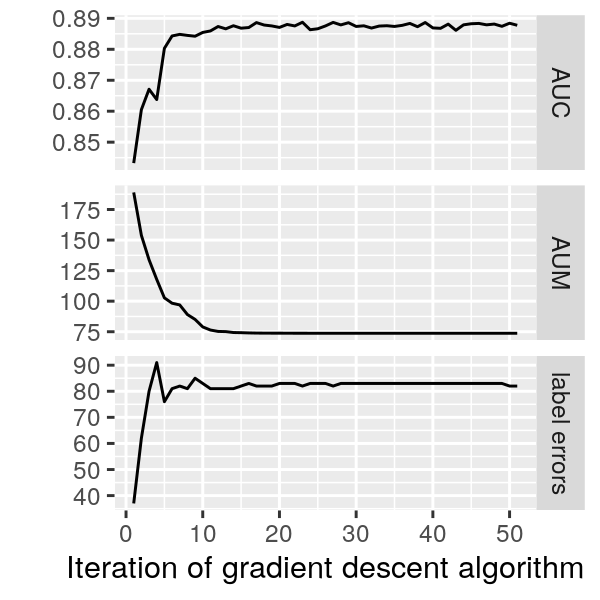
\includegraphics[height=6cm]{figure-aum-optimized-iterations.png}
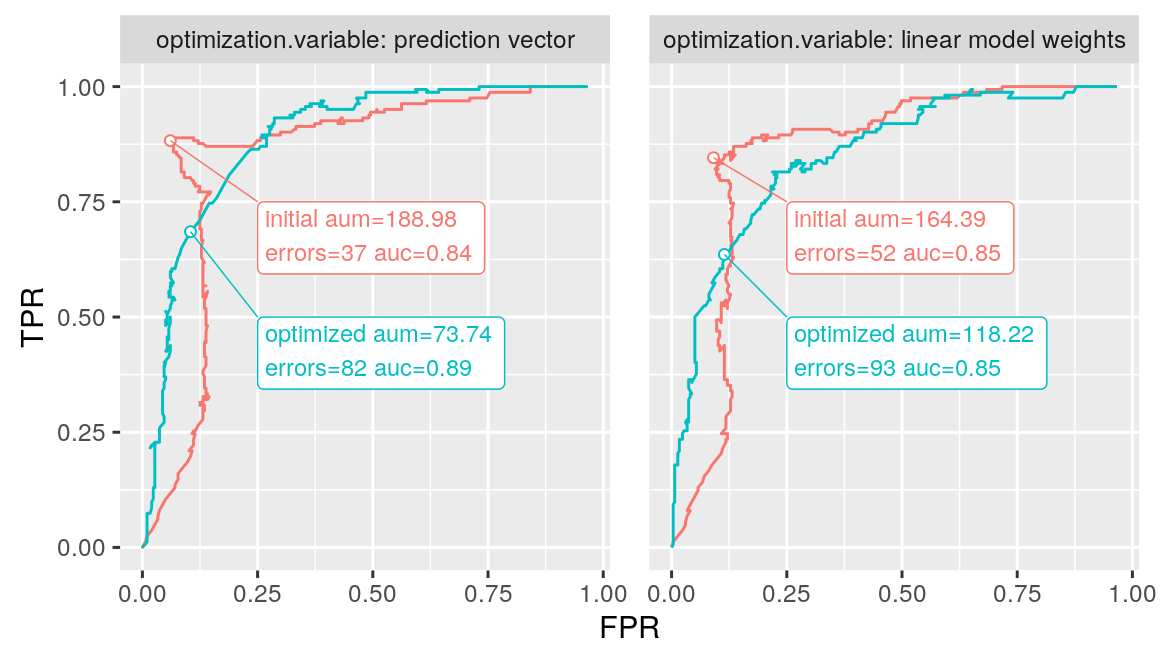
\includegraphics[height=6cm]{figure-aum-train-both.png}
\vskip -0.5cm
\caption{
Minimizing the AUM tends to increase AUC and label error rates, with respect to the train set ($n=54$ labeled examples).
\textbf{Left:} we used AUM gradient descent on the $n$-vector of predicted values $\mathbf{\hat y}$ in the train set (initial predictions chosen by minimizing label errors for each example). Decreases in AUM happen during the same iterations as increases in AUC and label error rates. 
\textbf{Middle:} ROC curves before and after using AUM gradient descent on the $n$-vector of predicted values (dot shows the point on each ROC curve with minimum label errors).
\textbf{Right:} optimizing the $p$-vector of weights in a linear model ($p=27$ features, initial weights minimize an un-regularized squared hinge loss). 
Note that AUC=0.85 is unchanged by the optimization but AUM decreases and error rate increases.
}
\label{fig:aum-optimized}
\end{center}
\vskip -0.2in
\end{figure*}

\section{Empirical Results}
\label{sec:results}
We empirically study AUM minimization in the context of changepoint detection problems, because they have non-monotonic FP and FN functions.
Our goal is to demonstrate that AUM minimization can result in AUC maximization with respect to train and test data.
\subsection{AUM gradient descent optimizes train AUC}

In this experiment our goal was to demonstrate that minimizing the AUM results in maximizing the AUC in the train set. 
We used the UCI chipseq data (a benchmark for labeled changepoint detection), treating each (set.name, fold) as a different train set, with pre-processing as previously described.\footnote{
\url{https://github.com/tdhock/feature-learning-benchmark}}
In brief, for each labeled example, changepoint models were computed for a range of penalty values, which resulted in models with a range of changepoints (some with few changepoints, others with many).
Then the label error rate for each model was computed, along with a penalty $\hat \lambda_i$ which resulted in minimum label errors for each labeled example $i$.
Finally these penalty values were used as the initial prediction vector $\mathbf{\hat y} = [ -\log\hat\lambda_1 \cdots -\log\hat\lambda_n]$, which was used as the optimization variable in an AUM gradient descent algorithm. 
A line search was used for the step size so that the AUM was guaranteed to decrease at each iteration. 
Overall there were 68 different train sets with the number of labeled examples ranging from $n=7$ to 1011.
% > fold.counts[, list(
% +   folds=.N,
% +   min.examples=min(examples),
% +   max.examples=max(examples)
% + )]
%   folds min.examples max.examples
% 1:    68            7         1011

We expected that by using the predicted values directly as the optimization variable in gradient descent, we should be able to obtain ROC curves that were significantly different from the initialization (hopefully with larger AUC, even though the initialization came from minimizing the label error independently for each example).
In a small number of train sets we observed that the optimization resulted in little or no change to both AUM and AUC; this happened when the initialization was close to or at a stationary point of the AUM (e.g., when AUM=0 and AUC=1).
However in most of the train sets we observed that minimizing the AUM results in increased AUC (on the train set). 
                    % set.name fold examples labels
% 64:        H3K4me3_XJ_immune    4       54    351
In one representative train set (H3K4me3\_XJ\_immune fold 4 which has $n=54$ labeled examples), we observed that the AUC and label error rate increases during the same iterations that the AUM decreases (Figure~\ref{fig:aum-optimized}, left).
Before optimization the ROC curve was highly non-monotonic with a sharp point in the upper left corner; after AUM optimization the ROC curve became more regular with increased area (Figure~\ref{fig:aum-optimized}, middle).
This result suggests that AUM gradient descent can be used to maximize the AUC, although the label error rate also increases.

We performed a second experiment, this time optimizing  $p=27$ weights in a linear model parameter vector which was used to compute a prediction for each of the $n=54$ labeled examples.
The weights were initialized by using a gradient descent algorithm to minimize an un-regularized squared hinge loss that is a convex relaxation of the label error \citep{Hocking2013icml}.
We expected the constraints of the linear model to reduce the accuracy with respect to the previous experiment (direct optimization of predicted values).
We observed that after optimizing the weights using AUM gradient descent, the train AUC remained the same, but the train error rate increased (Figure~\ref{fig:aum-optimized}, right).
This experiment shows that the constraints of a linear model can prevent AUM minimization from resulting in AUC maximization (even in a data set for which it is possible to achieve larger AUC values).

\subsection{Prediction accuracy and error in cross-validation}

TODO Jon changepoint data figure and discussion.



%TODO Binary classification?

\begin{figure*}[ht]
\vskip 0.2in
\begin{center}
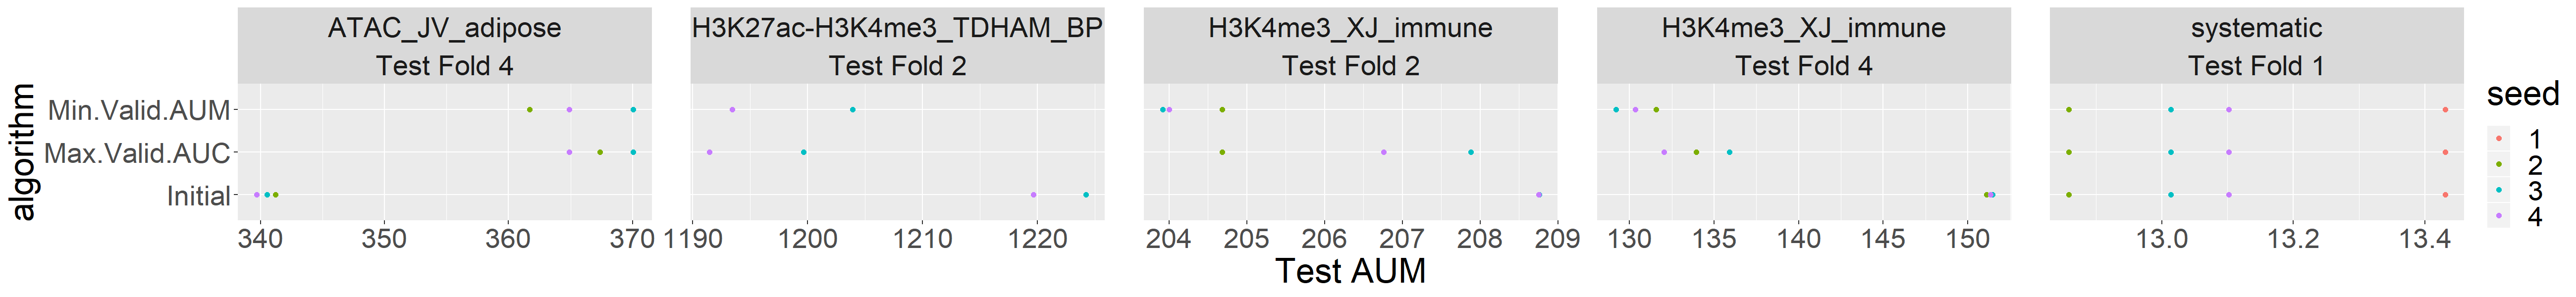
\includegraphics[width=\textwidth]{figure-test-aum-comparison.png}
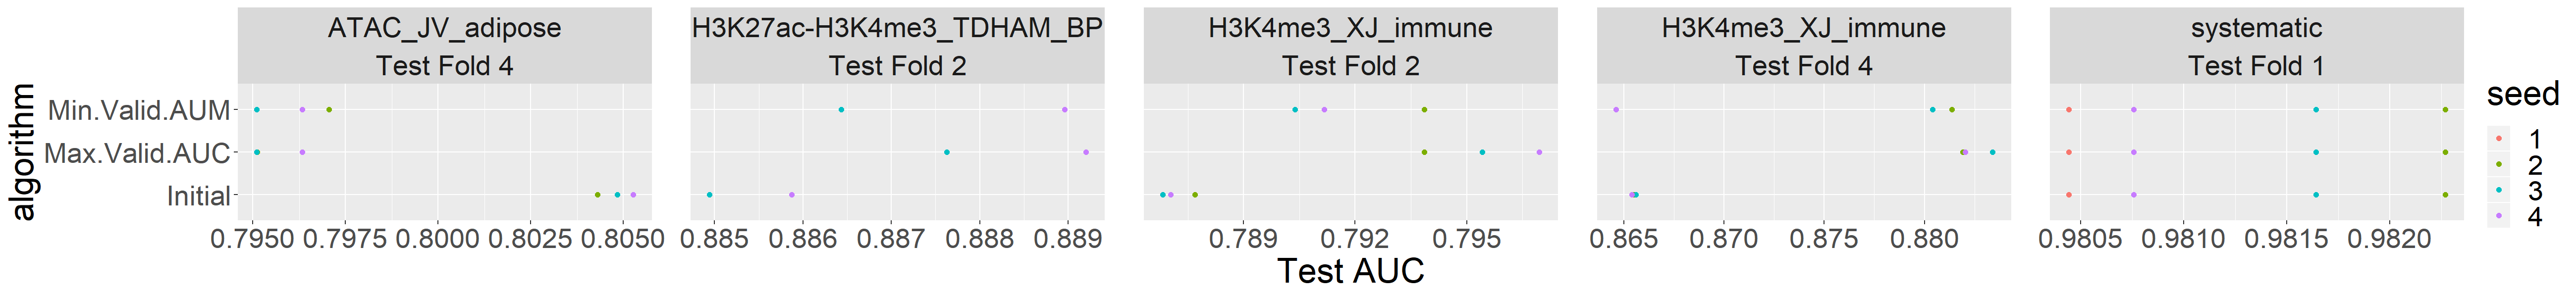
\includegraphics[width=\textwidth]{figure-test-auc-comparison.png}
\vskip -0.5cm
\caption{Testing text}
\label{fig:test-aum-comparison}
\end{center}
\vskip -0.2in
\end{figure*}
\section{Discussion and conclusions}
\label{sec:discussion}

In this paper we proposed the new AUM loss function for supervised binary classification and changepoint detection problems.
We proposed a new algorithm for efficiently computing the AUM and its directional derivatives, then showed how the AUM can be directly optimized in a linear gradient descent learning algorithm. 

We have shown that in changepoint detection problems with non-monotonic FP/FN functions, there is a tradeoff between AUC and accuracy that does not exist in binary classification problems.
If maximizing accuracy with respect to the labels is important, we can use existing convex loss functions centered on the predicted values which maximize accuracy.
If maximizing AUC is important, then we can minimize our new AUM loss function which we have shown empirically results in AUC maximization (but lower accuracy).
This tradeoff between AUC and accuracy means that the max accuracy model results in a highly non-monotonic ROC curve with many sub-optimal points, whereas the max AUC model has a more regular ROC curve (Figure~\ref{fig:aum-optimized}).

% or variant which ignores the amount of threshold and instead counts number of thresholds (like ROC only depends on number of thresholds, not the amount) this would amount to removing the        $\tau(\mathbf {\hat y})_{q} - \tau(\mathbf {\hat y})_{q-1}$ term in (\ref{eq:AUM-computation}) -> would not work, piecewise constant so not differentiable, can't use gradient descent.

For future work, we would like to consider several variants of our new AUM loss function.
In this work we defined the AUM as the area under the minimum of false positive and false negative \emph{counts}, but we could instead use \emph{rates} which would correspond to assigning equal weights to the two classes of errors.
In this work we proposed a full gradient algorithm (takes a step defined by all training examples), and we would additionally like to explore a batch variant (takes a step defined by a subset of training examples).
Finally our current algorithm uses a grid search over step sizes to perform the line search, but that could perhaps be improved by exploiting the piecewise linear nature of the AUM.
%area under something else (maybe remove all ROC points which are sub-optimal to some other point in either FPR or TPR).

\section*{Software and Data}

All of the software and data required to make the figures in this paper can be downloaded from URL HIDDEN DURING PEER REVIEW. An R package which implements the AUM gradient computation is available at URL HIDDEN DURING PEER REVIEW.

% Acknowledgements should only appear in the accepted version.
% \section*{Acknowledgements}

% \textbf{Do not} include acknowledgements in the initial version of
% the paper submitted for blind review.

% If a paper is accepted, the final camera-ready version can (and
% probably should) include acknowledgements. In this case, please
% place such acknowledgements in an unnumbered section at the
% end of the paper. Typically, this will include thanks to reviewers
% who gave useful comments, to colleagues who contributed to the ideas,
% and to funding agencies and corporate sponsors that provided financial
% support.


\bibliography{refs}
\bibliographystyle{icml2021}

\end{document}
